\section{Belzel}

%AGGIUNTA IMMAGINE NELLA MINIPAGE
%% \begin{figure}[H]
%%   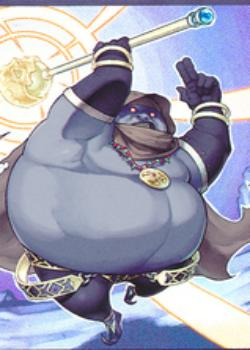
\includegraphics{Images/Characters/belzel}
%%   %Teniamo questo caption e in futuro mettiamo caption di questo stile quando ci realizzerà qualcosa
%%   \caption{Sketch of Belzel made by Elena Coperchini}
%% \end{figure}

\begin{minipage}{0.5\textwidth}
\textbf{Name}: Belzel \\
\textbf{Function}: Helper

\subsection{Internal World}

\textbf{Age \& Gender}: about 350, Male \\
\textbf{Values \& Virtues}: Man of his word  \\
\textbf{Personality}: Quiet, loner, helpful, kind \\
\textbf{Interests}: Meditation, inner peace \\
\textbf{Ethnic Group}: Arabic djinn

\subsection{External World}
\textbf{Environment}: Desert in the south of Ingary  \\
\textbf{Education}: High-educated, magic \\
\textbf{Social \& Cultural Background}: He has left society many decades ago and he is used to live alone \\
\textbf{Look \& Feel}: He looks like a 50-years-old fat man with long beard \\
\textbf{Job \& Experience}: He is a powerful wizard \\

\end{minipage}%
%
\hfill\begin{minipage}{0.4\textwidth}
  \begin{figure}[H]
    \hfill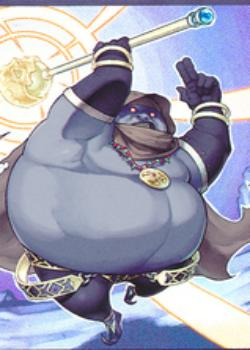
\includegraphics{Images/Characters/belzel}
    \caption{Sketch of Belzel made by Elena Coperchini}
  \end{figure}
\end{minipage}

%% QUESTE INFORMAZIONI SONO STATE AGGIUNTE NELLA MINIPAGE
%% \textbf{Name}: Belzel \\
%% \textbf{Function}: Helper

%% \subsection{Internal World}
%% \textbf{Age \& Gender}: 347, Male \\
%% \textbf{Values \& Virtues}: Man of his word  \\
%% \textbf{Personality}: Quiet, loner, helpful, kind \\
%% \textbf{Interests}: Meditation, inner peace \\
%% \textbf{Ethnic Group}: Arabic Djinn

%% \subsection{External World}
%% \textbf{Environment}: Desert in the South of Ingary.  \\
%% \textbf{Education}: High-educated. \\
%% \textbf{Social \& Cultural Background}: He has left society many decades ago and he is used to live alone. \\
%% \textbf{Look \& Feel}: He looks like a 50-years-old fat man with long beard. \\
%% \textbf{Job \& Experience}: He is a powerful wizard. \\

\subsubsection*{Relationships}
\begin{itemize}
\item \textbf{Sophie and Calcifer}: He is glad to help them because he feels they really need his help.
\item \textbf{Howl, Justin, Suliman, Mizar}: No one knows each other.
\end{itemize}

\begin{figure}[H]
  \centering
  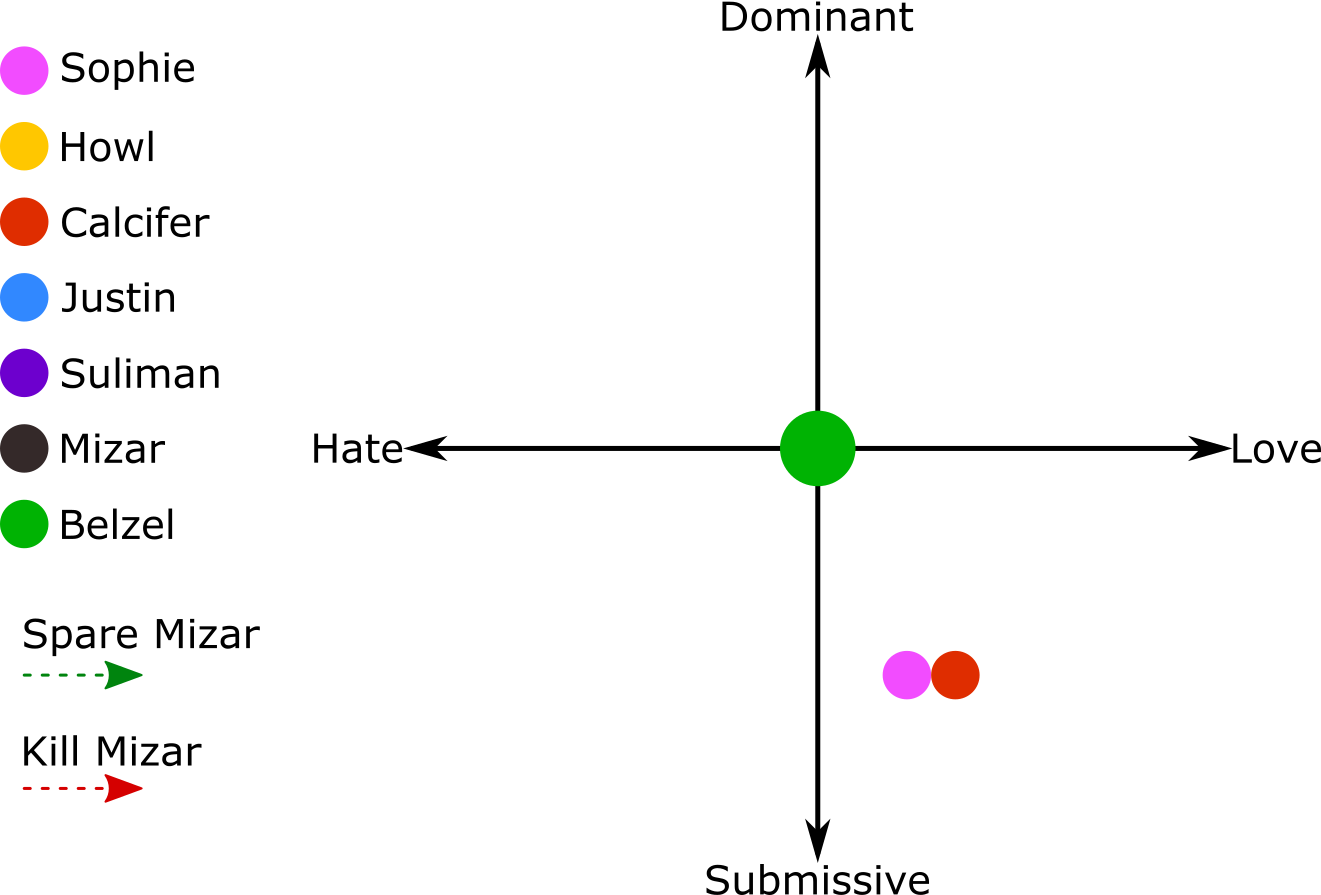
\includegraphics[width=8cm]{Images/SVG/Exported/Circumplexes/belzelCircumplex}
  \caption{Circumplex of Belzel}
\end{figure}

\begin{figure}[H]
   \centering
   
\includegraphics[width=8cm]{Images/SVG/Exported/Evolutions/belzelEvolution}
   \caption{Evolutions of Belzel}
\end{figure}

\subsection{Description}
He is a djinn who spends his days meditating and practicing with new spells. He loves being helpful for people who actually need his help.

\subsection{Background story}
He decided to move many decades ago into the desert because he felt like the society he was living in was too selfish and asked him for help only for futile things.

Nowadays, no one knows him personally but people in the south of Ingary think, according to a common legend, that he still lives alone in the desert and he helps people when they are really in trouble.
